\section{Motivation}

\logo{}

\begin{frame}
    \frametitle{Forecast combination - point and density}

    Forecast tomorrow's temperature
    
    \begin{columns}[t]
    \begin{column}{0.4\textwidth}
        \begin{exampleblock}{Model 1}
        Classical Linear Regression Model
        \end{exampleblock}
    \end{column}
    
    \begin{column}{0.5\textwidth}
        \begin{exampleblock}{Model 2}
        Autoregressive Integrated Moving Average Model
        \end{exampleblock}
    \end{column}
    \end{columns}

    \vspace{5mm}
    
    Combining multiple forecasts can dramatically improve the forecast accuracy (\cite{BG69}).

\begin{figure}[b]
\centering
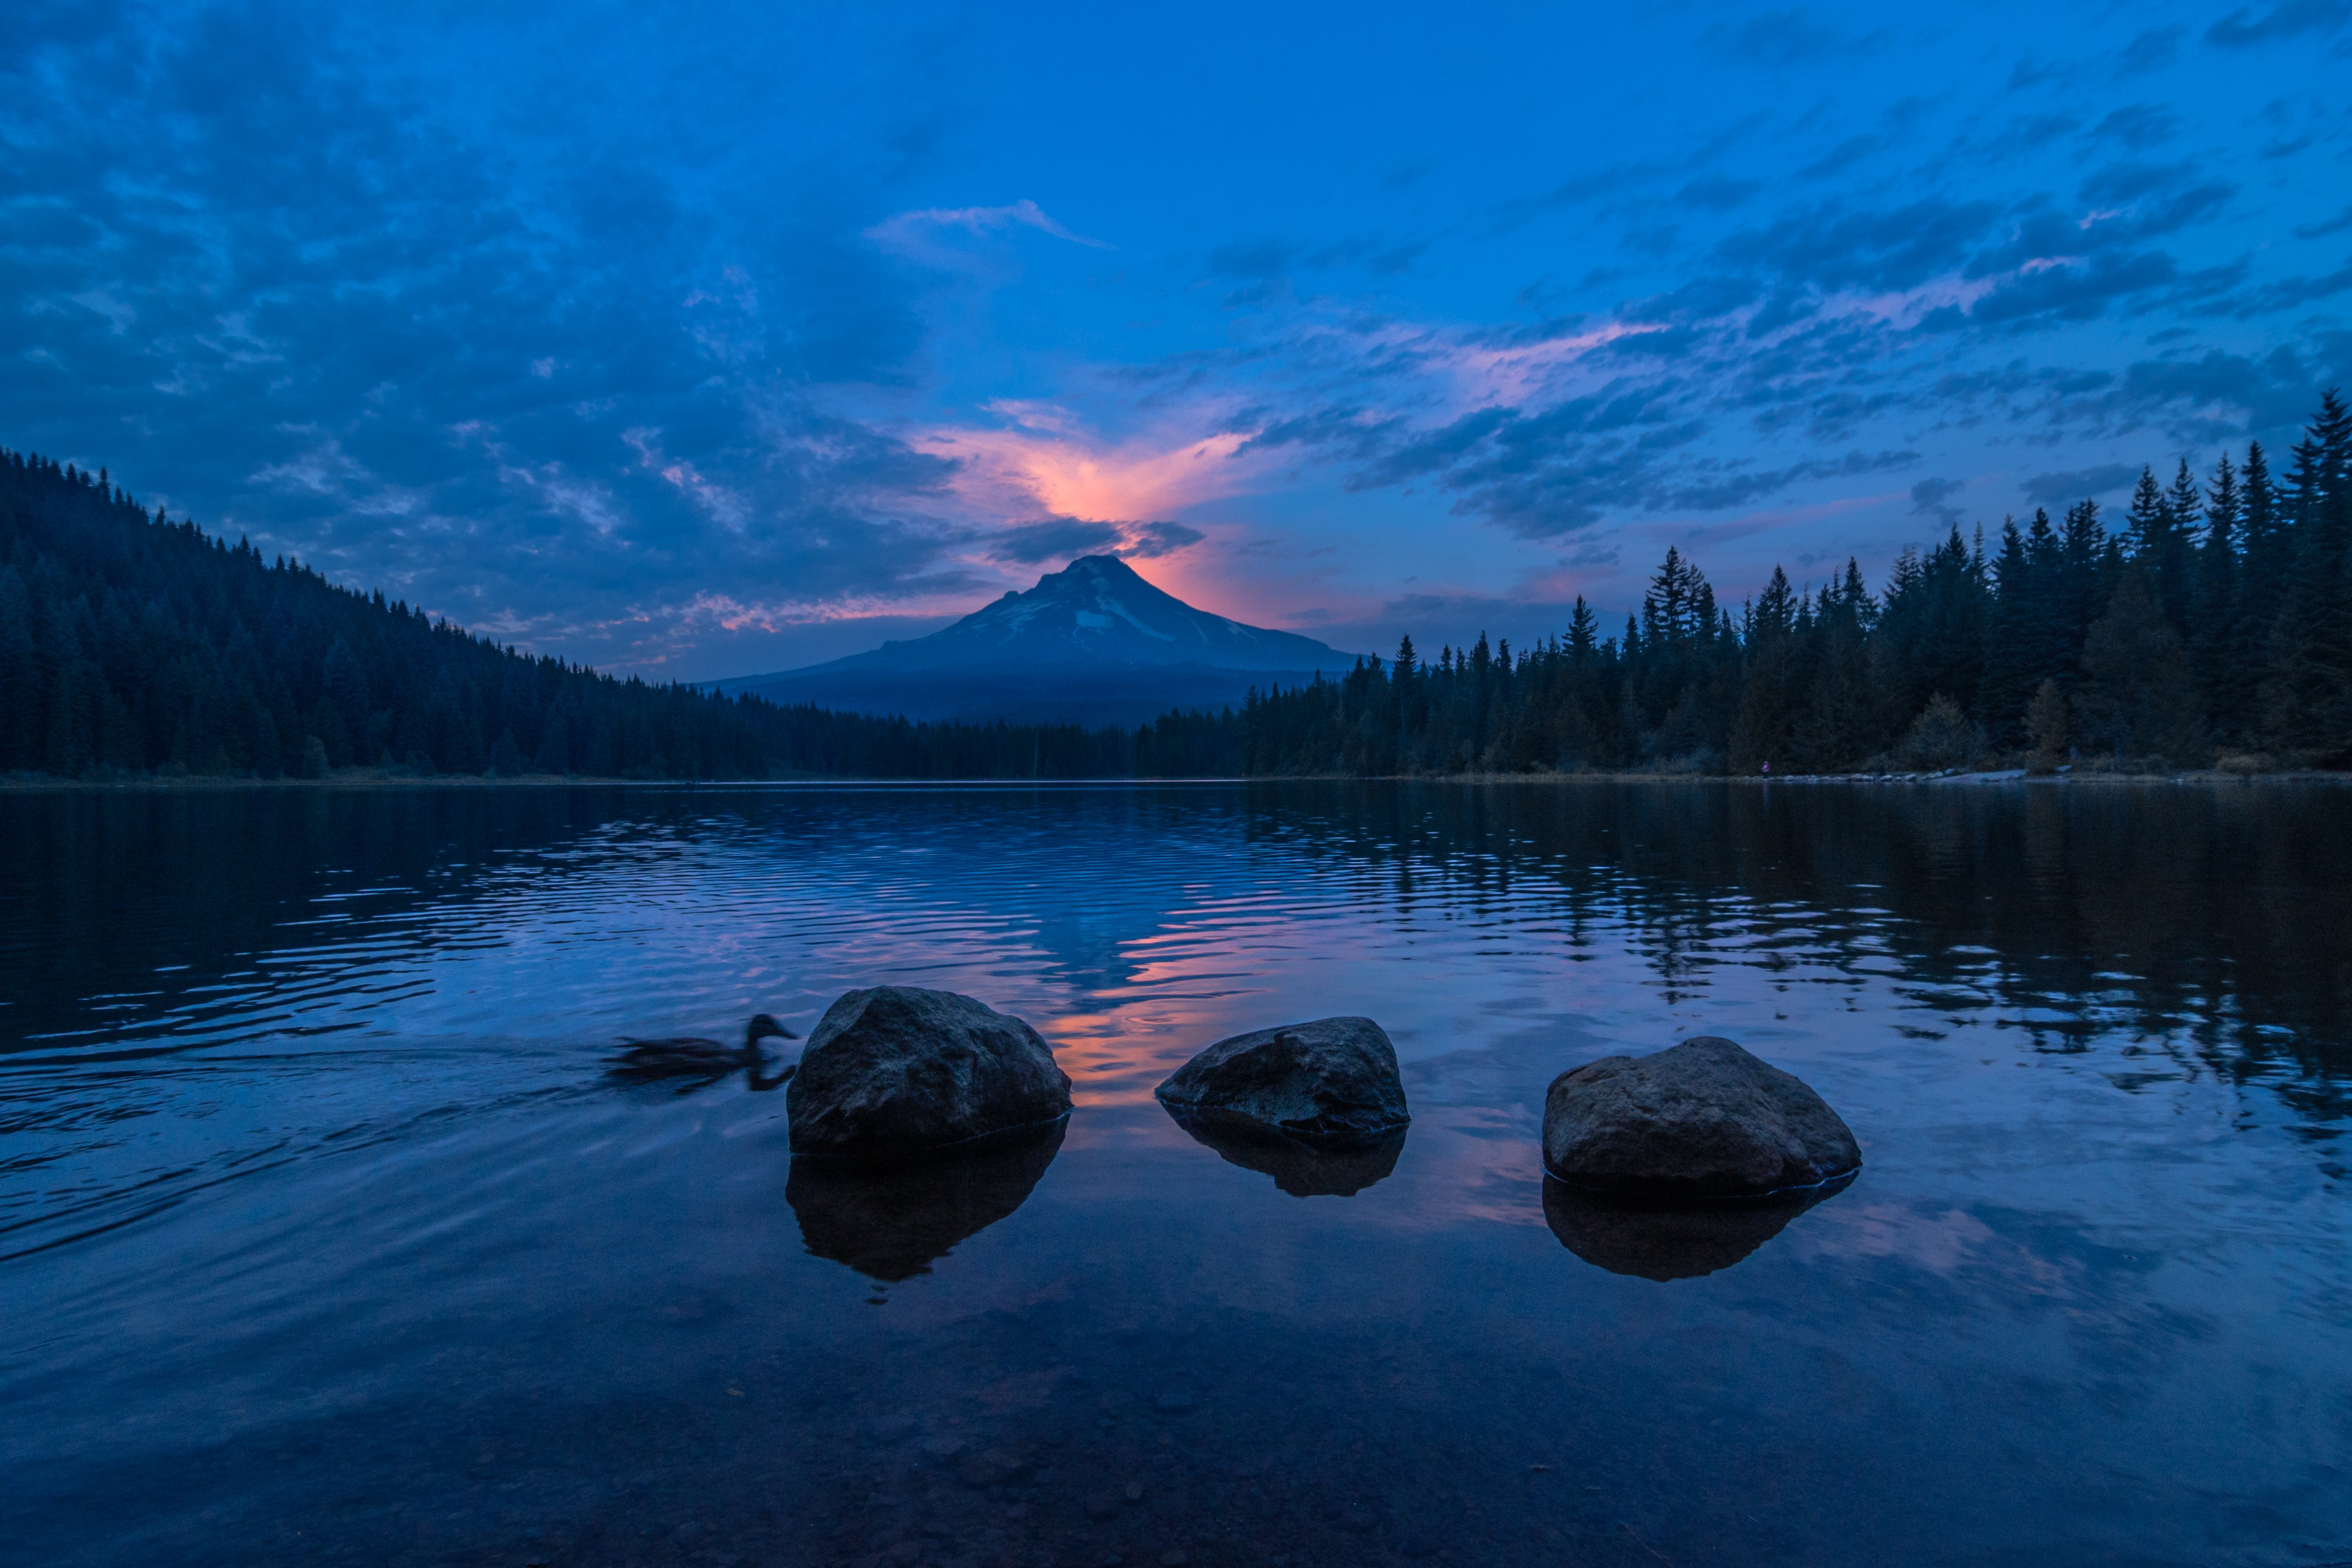
\includegraphics[width=3cm]{Graph/Weather.jpg}
\end{figure}

\end{frame}

\begin{frame}
\frametitle{What is the forecast combination puzzle?}

    The puzzle refers to the empirical finding that an equally weighted combination of forecasts generally outperforms more sophisticated combination schemes.

    \vspace{5mm}

    \textit{“Theoretically sophisticated weighting schemes should provide more benefits than the sample average from forecast combination, while empirically the simple average has been continuously found to dominate more complicated approaches to combining forecasts” (\cite{WHLK22}).}

        \begin{columns}[t]
    \begin{column}{0.4\textwidth}
        \begin{block}{}
        \centering
        Simple Averaging \\
        / Equal Weights
        \end{block}
    \end{column}
    
    \begin{column}{0.5\textwidth}
        \begin{block}{}
        \centering
        Complicated Weighting Schemes
        \end{block}
    \end{column}
    \end{columns}
    
\end{frame}


\begin{frame}
    \frametitle{Explanations of the puzzle in literature}

        \begin{exampleblock}{\Large{Uncertainty in Weight Estimation}}
        \cite{SW98}, \cite{SW04}, and \cite{SW09}
        \end{exampleblock}

        \vspace{8mm}

        \begin{exampleblock}{\Large{Trade-off between Bias and Variance}}
        \cite{E11} and \cite{CMVW16}
        \end{exampleblock}

\end{frame}



\begin{frame}
\frametitle{A Recent Explanation}

    \begin{alertblock}{\Large{Estimation Uncertainty of Forecasts}}
    \cite{ZMFP22} and \cite{FZMP23}
    \end{alertblock}

    \vspace{5mm}
    
    They proposed a new aspect of explanation by investigating the sampling variability in model estimation. They illustrated that, asymptotically, the bias and variability mainly come from the estimation of forecasts.

\end{frame}





